\documentclass[14pt]{extbook}
\usepackage{multicol, enumerate, enumitem, hyperref, color, soul, setspace, parskip, fancyhdr} %General Packages
\usepackage{amssymb, amsthm, amsmath, bbm, latexsym, units, mathtools} %Math Packages
\everymath{\displaystyle} %All math in Display Style
% Packages with additional options
\usepackage[headsep=0.5cm,headheight=12pt, left=1 in,right= 1 in,top= 1 in,bottom= 1 in]{geometry}
\usepackage[usenames,dvipsnames]{xcolor}
\usepackage{dashrule}  % Package to use the command below to create lines between items
\newcommand{\litem}[1]{\item#1\hspace*{-1cm}\rule{\textwidth}{0.4pt}}
\pagestyle{fancy}
\lhead{Progress Quiz 3}
\chead{}
\rhead{Version C}
\lfoot{3148-2249}
\cfoot{}
\rfoot{Spring 2021}
\begin{document}

\begin{enumerate}
\litem{
Construct the lowest-degree polynomial given the zeros below. Then, choose the intervals that contain the coefficients of the polynomial in the form $x^3+bx^2+cx+d$.\[ -2 - 5 i \text{ and } -3 \]\begin{enumerate}[label=\Alph*.]
\item \( b \in [-13, -2], c \in [40, 42.8], \text{ and } d \in [-90, -77] \)
\item \( b \in [-3, 2], c \in [3.1, 6.1], \text{ and } d \in [-1, 8] \)
\item \( b \in [6, 10], c \in [40, 42.8], \text{ and } d \in [84, 96] \)
\item \( b \in [-3, 2], c \in [5.5, 10.3], \text{ and } d \in [13, 21] \)
\item \( \text{None of the above.} \)

\end{enumerate} }
\litem{
Construct the lowest-degree polynomial given the zeros below. Then, choose the intervals that contain the coefficients of the polynomial in the form $ax^3+bx^2+cx+d$.\[ \frac{-3}{2}, \frac{-5}{4}, \text{ and } \frac{7}{4} \]\begin{enumerate}[label=\Alph*.]
\item \( a \in [26, 33], b \in [-38, -30], c \in [-101, -92], \text{ and } d \in [105, 110] \)
\item \( a \in [26, 33], b \in [32, 36], c \in [-101, -92], \text{ and } d \in [-111, -104] \)
\item \( a \in [26, 33], b \in [32, 36], c \in [-101, -92], \text{ and } d \in [105, 110] \)
\item \( a \in [26, 33], b \in [-144, -138], c \in [207, 217], \text{ and } d \in [-111, -104] \)
\item \( a \in [26, 33], b \in [-72, -58], c \in [-56, -45], \text{ and } d \in [105, 110] \)

\end{enumerate} }
\litem{
Which of the following equations \textit{could} be of the graph presented below?
\begin{center}
    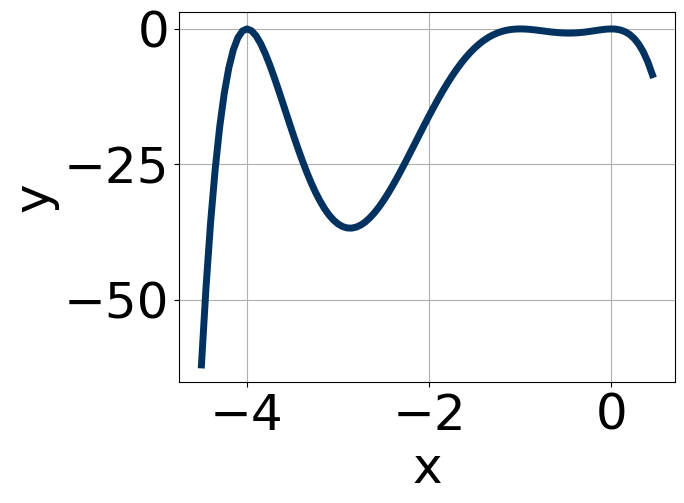
\includegraphics[width=0.5\textwidth]{../Figures/polyGraphToFunctionC.png}
\end{center}
\begin{enumerate}[label=\Alph*.]
\item \( -13x^{6} (x + 3)^{7} (x - 2)^{10} \)
\item \( 12x^{10} (x + 3)^{9} (x - 2)^{11} \)
\item \( -3x^{6} (x + 3)^{5} (x - 2)^{5} \)
\item \( 15x^{7} (x + 3)^{10} (x - 2)^{5} \)
\item \( 19x^{10} (x + 3)^{8} (x - 2)^{9} \)

\end{enumerate} }
\litem{
Describe the end behavior of the polynomial below.\[ f(x) = 7(x - 9)^{5}(x + 9)^{8}(x + 2)^{4}(x - 2)^{4} \]\begin{enumerate}[label=\Alph*.]
\begin{multicols}{2}\item 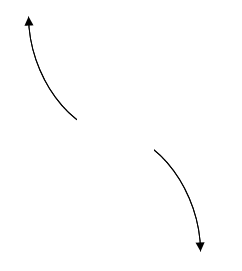
\includegraphics[width = 0.3\textwidth]{../Figures/polyEndBehaviorCopyAC.png}\item 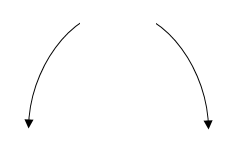
\includegraphics[width = 0.3\textwidth]{../Figures/polyEndBehaviorCopyBC.png}\item 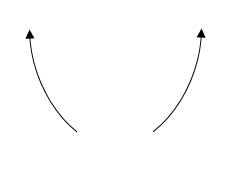
\includegraphics[width = 0.3\textwidth]{../Figures/polyEndBehaviorCopyCC.png}\item 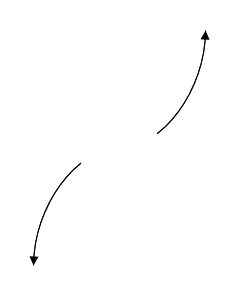
\includegraphics[width = 0.3\textwidth]{../Figures/polyEndBehaviorCopyDC.png}\end{multicols}\item None of the above.
\end{enumerate} }
\litem{
Construct the lowest-degree polynomial given the zeros below. Then, choose the intervals that contain the coefficients of the polynomial in the form $ax^3+bx^2+cx+d$.\[ -3, \frac{2}{3}, \text{ and } -7 \]\begin{enumerate}[label=\Alph*.]
\item \( a \in [3, 5], b \in [-28.7, -25.9], c \in [42, 48], \text{ and } d \in [41, 44] \)
\item \( a \in [3, 5], b \in [13.4, 15.1], c \in [-56, -54], \text{ and } d \in [-42, -41] \)
\item \( a \in [3, 5], b \in [6.1, 12.1], c \in [-75, -70], \text{ and } d \in [41, 44] \)
\item \( a \in [3, 5], b \in [27.6, 30.4], c \in [42, 48], \text{ and } d \in [-42, -41] \)
\item \( a \in [3, 5], b \in [27.6, 30.4], c \in [42, 48], \text{ and } d \in [41, 44] \)

\end{enumerate} }
\litem{
Which of the following equations \textit{could} be of the graph presented below?
\begin{center}
    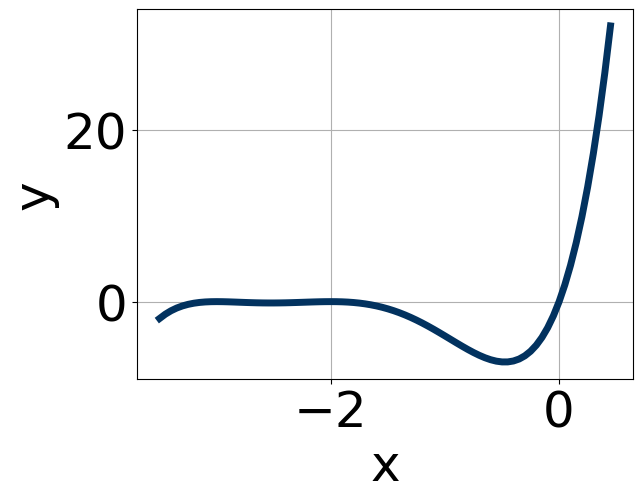
\includegraphics[width=0.5\textwidth]{../Figures/polyGraphToFunctionCopyC.png}
\end{center}
\begin{enumerate}[label=\Alph*.]
\item \( -14x^{5} (x + 4)^{10} (x + 3)^{11} \)
\item \( -15x^{6} (x + 4)^{8} (x + 3)^{5} \)
\item \( 18x^{11} (x + 4)^{4} (x + 3)^{7} \)
\item \( 12x^{11} (x + 4)^{10} (x + 3)^{10} \)
\item \( 5x^{11} (x + 4)^{9} (x + 3)^{4} \)

\end{enumerate} }
\litem{
Describe the zero behavior of the zero $x = 7$ of the polynomial below.\[ f(x) = 3(x - 7)^{8}(x + 7)^{11}(x + 5)^{3}(x - 5)^{4} \]\begin{enumerate}[label=\Alph*.]
\begin{multicols}{2}\item 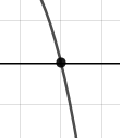
\includegraphics[width = 0.3\textwidth]{../Figures/polyZeroBehaviorAC.png}\item 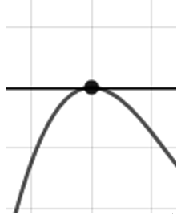
\includegraphics[width = 0.3\textwidth]{../Figures/polyZeroBehaviorBC.png}\item 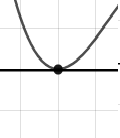
\includegraphics[width = 0.3\textwidth]{../Figures/polyZeroBehaviorCC.png}\item 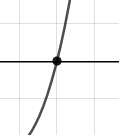
\includegraphics[width = 0.3\textwidth]{../Figures/polyZeroBehaviorDC.png}\end{multicols}\item None of the above.
\end{enumerate} }
\litem{
Construct the lowest-degree polynomial given the zeros below. Then, choose the intervals that contain the coefficients of the polynomial in the form $x^3+bx^2+cx+d$.\[ 4 - 3 i \text{ and } 1 \]\begin{enumerate}[label=\Alph*.]
\item \( b \in [-4, 3], c \in [1, 7], \text{ and } d \in [-6, -1] \)
\item \( b \in [-4, 3], c \in [-11, -3], \text{ and } d \in [1, 6] \)
\item \( b \in [-10, -7], c \in [31, 38], \text{ and } d \in [-25, -20] \)
\item \( b \in [3, 13], c \in [31, 38], \text{ and } d \in [14, 32] \)
\item \( \text{None of the above.} \)

\end{enumerate} }
\litem{
Describe the zero behavior of the zero $x = 7$ of the polynomial below.\[ f(x) = -8(x - 5)^{10}(x + 5)^{8}(x - 7)^{11}(x + 7)^{6} \]\begin{enumerate}[label=\Alph*.]
\begin{multicols}{2}\item 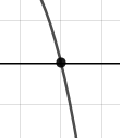
\includegraphics[width = 0.3\textwidth]{../Figures/polyZeroBehaviorCopyAC.png}\item 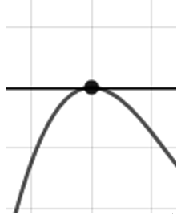
\includegraphics[width = 0.3\textwidth]{../Figures/polyZeroBehaviorCopyBC.png}\item 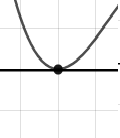
\includegraphics[width = 0.3\textwidth]{../Figures/polyZeroBehaviorCopyCC.png}\item 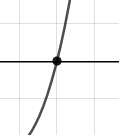
\includegraphics[width = 0.3\textwidth]{../Figures/polyZeroBehaviorCopyDC.png}\end{multicols}\item None of the above.
\end{enumerate} }
\litem{
Describe the end behavior of the polynomial below.\[ f(x) = 8(x + 6)^{5}(x - 6)^{10}(x + 8)^{2}(x - 8)^{2} \]\begin{enumerate}[label=\Alph*.]
\begin{multicols}{2}\item 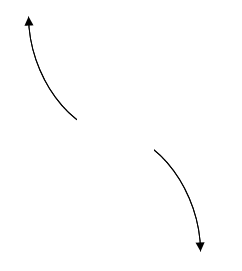
\includegraphics[width = 0.3\textwidth]{../Figures/polyEndBehaviorAC.png}\item 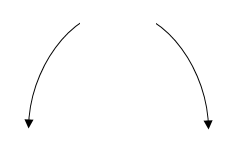
\includegraphics[width = 0.3\textwidth]{../Figures/polyEndBehaviorBC.png}\item 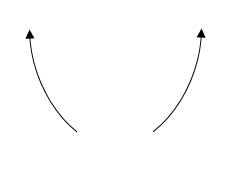
\includegraphics[width = 0.3\textwidth]{../Figures/polyEndBehaviorCC.png}\item 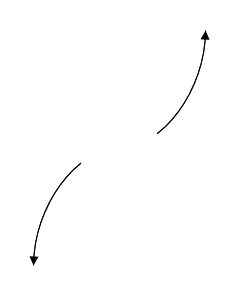
\includegraphics[width = 0.3\textwidth]{../Figures/polyEndBehaviorDC.png}\end{multicols}\item None of the above.
\end{enumerate} }
\end{enumerate}

\end{document}